\section{Bootloader}
Il bootloader è un software che si trova in memoria flash e si occupa di prendere del codice da una periferica e di scriverlo in flash con l' istruzione SPM:
\begin{figure}[H]
    \centering
    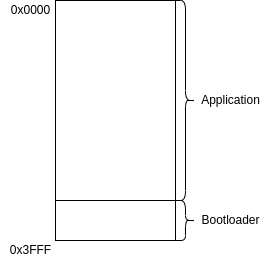
\includegraphics[width=150px]{images/27_Bootloader/bootloader.png}
\end{figure}
Arduino ad esempio utilizza un custom bootloader per permettere la programmazione attraverso la USART, in questo modo la programmazione è semplice e non richiede hardware esterno particolare.

Dal momento che alla partenza del uC parte il codice all' indirizzo 0x0000 bisogna programmare l' applicazione in modo che riconosca una particolare sequenza per passare il controllo al bootloader.
Questo sistema tuttavia è poco affidabile in quanto ci sono vari modi di rompere le cose.

L' ideale pertanto è chiamare sempre il bootloader all' avvio, attendere per la sequenza specifica e successivamente andare all' applicazione.
Per fare ciò scriviamo nel vettore di reset l' indirizzo del bootloader.

Per come è strutturata la programmazione della flash non possiamo leggerla mentre la scriviamo, per questo motivo la flash è divisa in due zone differenti in modo che se scrivo nella zona applicazione posso eseguire il bootloader, mentre se scrivo nel bootloader non posso eseguire niente.
Si dice che la sezione applicazione è \emph{read while write} mentre la sezione bootloader è \emph{no read while write}.

Il confine tra le due zone si può scegliere con dei fusibili per allargare più o meno il bootloader.

Per eseguire una scrittura nella flash si usa l' istruzione SPM e per sapere lo stato della scrittura si usa il registro SPMCR.
La scrittura in flash è lenta (migliaia di cicli di clock) quindi si usa un interrupt per sapere quando finisce oppure testare in continuazione in loop il bit RWWSB.
Quando si scrive si scrive una intera pagina da 64 byte per volta in quanto si deve:
\begin{itemize}
    \item cancella una pagina (settare tutto ad 1)
    \item scrivere il contenuto nella RAM
    \item dire di copiare i dati dalla RAM alla FLASH
\end{itemize}
di solito coviene anche leggere ciò che si è appena scritto nella FLASH e compararlo con quanto scritto nella RAM in modo da accorgersi di eventuali problemi nella programmazione, questi possono avvenire in seguito a tante riscritture dato che le memorie FLASH hanno un numero massimo di scritture fattibili prima che il chip smetta di funzionare adeguatamente.

\subsection{SPMCR}
\begin{figure}[H]
    \centering
    
\includegraphics[width=330px]{images/27_Bootloader/SPMCR.png}
\end{figure}
\begin{itemize}
    \item PGWRT: scrivendoci 1 assieme a SPMEN ed eseguendo una SPM nei 4 cicli di clock successivi avvia la scrittura nella FLASH

    \item SPMEN: abilita la scrittura se si esegue una SPM nei 4 cicli di clock successivi

    \item PGERS: scrivendoci 1 assieme a SPMEN ed eseguendo una SPM nei 4 cicli di clock successivi avvia la cancellazione di una pagina di FLASH
\end{itemize}
l' indirizzo della pagina sulla quale eseguire le operazioni si inserisce nei registri ZH:ZL.


